\documentclass[12pt, a4paper]{article}

\usepackage[utf8]{inputenc}
\usepackage[T1]{fontenc}
\usepackage[russian]{babel}
\usepackage[oglav,spisok,boldsect,eqwhole,figwhole,hyperref,hyperprint,remarks,greekit]{./style/fn2kursstyle}
\usepackage{tikz}
\graphicspath{{./style/}{./figures/}}

\usepackage{multirow}
\usepackage{supertabular}
\usepackage{multicol}
\usepackage{mathtools}
% Параметры титульного листа
\title{Прямые методы решения систем
	линейных алгебраических уравнений}
\lab{1}
\author{И.\,Е.~Дыбко}
\creator{С.\,И.~Тихомиров}
\supervisor{А.\,О.~Гусев}
\group{ФН2-51Б}
\date{2024}

% Переопределение команды \vec, чтобы векторы печатались полужирным курсивом
\renewcommand{\vec}[1]{\text{\mathversion{bold}${#1}$}}%{\bi{#1}}
\newcommand\thh[1]{\text{\mathversion{bold}${#1}$}}
%Переопределение команды нумерации перечней: точки заменяются на скобки
\renewcommand{\labelenumi}{\theenumi)}
\begin{document}
	
	\maketitle
	
	\tableofcontents
	\section{Описание использованных алгоритмов}
	
	\subsection{Метод Гаусса}		
	Для начала представим систему в виде расширенной матрицы. СЛАУ запишем в виде матрицы коэффициентов с добавлением столбца свободных членов (расширенная матрица).
	\begin{equation*}
		\begin{cases}
			a_{11}x_1 + a_{12}x_2 + \dots + a_{1n}x_n = b_1 \\
			a_{21}x_1 + a_{22}x_2 + \dots + a_{2n}x_n = b_2 \\
			\vdots \\
			a_{m1}x_1 + a_{m2}x_2 + \dots + a_{mn}x_n = b_m
		\end{cases}
	\end{equation*}
	
	Соответствующая расширенная матрица будет:
	\begin{equation*}
		\begin{pmatrix}
			a_{11} & a_{12} & \dots & a_{1n} & | & b_1 \\
			a_{21} & a_{22} & \dots & a_{2n} & | & b_2 \\
			\vdots & \vdots & \ddots & \vdots & | & \vdots \\
			a_{m1} & a_{m2} & \dots & a_{mn} & | & b_m
		\end{pmatrix}
	\end{equation*}
	
	Далее преобразуем расширенную матрицу к треугольному виду с нулями ниже главной диагонали. Цель — получить систему вида, где каждое уравнение имеет на одну переменную меньше:
	
	\begin{equation*}
		\begin{cases}
			x_1 + a_{12}'x_2 + \dots + a_{1n}'x_n = b_1' \\
			x_2 + a_{23}'x_3 + \dots + a_{2n}'x_n = b_2' \\
			\vdots \\
			x_n = b_n'
		\end{cases}
	\end{equation*}
	
	После того, как система приведена к треугольному виду, начинаем с последнего уравнения и поэтапно находим значения переменных:
	$$x_n = b_n'$$
	Подставляем $x_n$ в предыдущее уравнение, чтобы найти $x_{n-1}$, и так далее, пока не будут найдены все переменные.
	
	\subsection{Метод вращения Гивенса}
	
	Метод Гивенса используется для нахождения QR-разложения путём последовательного применения элементарных вращений (матриц Гивенса), которые зануляют элементы под диагональю. Вращения Гивенса -- это вращения в плоскости, которые применяются для зануления отдельных элементов матрицы, аналогично преобразованию отражений, но вращение воздействует только на две строки матрицы за раз.
	
	Матрица вращения Гивенса $G(i,j,\theta)$ -- это ортогональная матрица, которая зануляет элемент матрицы $A$ в позиции $a_{ij}$ (под диагональю), изменяя только строки $i$ и $j$. Выглядит она следующим образом:
	
	\begin{equation*}
		T_{ij} =
		\begin{pmatrix}
			1 & & & & & \\
			& \ddots & & & & \\
			& & c & \dots & s & \\
			& & \vdots & \ddots & \vdots & \\
			& & -s & \dots & c & \\
			& & & & & \ddots & \\
		\end{pmatrix},
	\end{equation*}
	где:
	$$c=\frac{a_{ii}}{\sqrt{a_{ii}^2+a_{ji}^2}}, \qquad s=\frac{a_{ji}}{\sqrt{a_{ii}^2+a_{ji}^2}}.$$
	
	Для каждого элемента под диагональю создаётся соответствующее вращение Гивенса. При умножении матрицы $A$ слева на матрицу $T_{ij}$, происходит зануление элемента $a_{ij}$. 
	
	Процесс последовательно повторяется для всех элементов под диагональю, в результате чего матрица $A$ становится верхнетреугольной "--- это и есть матрица $R$. Также, будем домножать слева  на $T_{ij}$  матрицу перехода $T$ (в начале матрицу $T$ положим единичной), таким образом: 
	\begin{equation*}
		T = T_{n-1, n} \cdot \ldots \cdot T_{24} \cdot T_{23} \cdot  T_{1,n} \cdot \ldots \cdot T_{13} \cdot T_{12}.
	\end{equation*}
Матрица $Q$ в свою очередь может быть найдена следующим образом: $Q=T^{-1}=T^{T}$. 

Таким образом исходная система преобразуется к следующему виду $Rx=b^{*}$, где $b^{*}=Tb$, для решения которой достаточно применить обратный ход Гаусса. 

	\section{Ответы на контрольные вопросы}
	\begin{enumerate}
		\item \textbf{Каковы условия применимости метода Гаусса без выбора
			и с выбором ведущего элемента?}
		
		\textbf{Без выбора ведущего элемента:} Метод Гаусса может быть применен, если на всех шагах на главной диагонали не возникает нулевых элементов: $$a^{(i-1)}_{ii}\ne 0, \quad  i = 1,2,\ldots,n.$$
		
		\textbf {С выбором ведущего элемента:} Метод с выбором ведущего элемента  применим всегда, когда матрица невырожденная ($\det A \ne 0$).
		
		\item \textbf{Докажите, что если $\det A \ne 0$, то при выборе главного
			элемента в столбце среди элементов, лежащих не выше главной диагонали, всегда найдется хотя бы один элемент, отличный от нуля.}
		
		Для любой невырожденной матрицы обязательно существует хотя бы один ненулевой элемент в каждом столбце среди элементов, которые находятся на главной диагонали или ниже ее. В противном случае хотя бы один столбец состоял бы из нулей, что привело бы к нулевому определителю, что противоречит условию ($\det A \ne 0$).
		
		
		\item \textbf{В методе Гаусса с полным выбором ведущего элемента приходится не только переставлять уравнения, но и менять нумерацию неизвестных. Предложите алгоритм, позволяющий восстановить первоначальный порядок неизвестных.}
		
		Создадим дополнительный одномерный массив \texttt{order\_arr}. Заполним его числами $0,1,2,\cdots, n-1$ по порядку. При перестановке переменных в дополнительном массиве будем менять элементы с соответствующими индексами. При выполнении элементарных преобразований, для того чтобы обратиться  к элементу в $i$-той строке и $j$-том столбце, нужно обратиться к элементу \texttt{A[i][order\_arr[j]]}.
		
		\item \textbf{Оцените количество арифметических операций, требуемых
			для QR-разложения произвольной матрицы $A$ размера $n \times n$.}
		\begin{enumerate}
			\item \textbf{ Метод Грамма"---Шмидта}
			
			Проекция вектора на другой вектор требует $2n$ операций. Для каждого из $n$ столбцов вычисляется $n-1$ проекций. Таким образом необходимо всего: 
			
			$$\sum = 2n (n-1) n = 2n^3 - 2n^2 \sim 2n^3.$$
			
			\item \textbf{ Метод отражений Хаусхолдера}
			
			Отражение Хаусхолдера для каждого столбца требует $2n^2$ операций, так как оно применяется ко всем элементам матрицы ниже диагонали. Для матрицы размером $n \times n$ таких отражений будет $n-1$. Таким образом необходимо всего: 
			$$\sum = 2n^2 (n-1) = 2n^3 - 2n^2 \sim 2n^3.$$
			\item \textbf{ Метод вращений Гивенса}
			
			Метод вращений Гивенса использует последовательные вращения для зануления элементов матрицы. Вращение затрагивает только два элемента одновременно, что делает метод особенно эффективным для разреженных матриц ($\sum = n^2$). Для плотных матриц, как правило, требуется также $\sum = n^3$ операций, так как необходимо применять множество вращений ко всем элементам матрицы.
		\end{enumerate}
		
		
		
		\item \textbf{Что такое число обусловленности и что оно характеризует?
			Имеется ли связь между обусловленностью и величиной
			определителя матрицы? Как влияет выбор нормы матрицы
			на оценку числа обусловленности?}
		
		Числом обусловленности $M_{A}=\|A^{-1}\| \|A\|$ называется числом обусловленности матрицы $A$ (и $A^{-1}$ в силу симметрии формулы). Оно характеризует, насколько сильно ошибка в данных может повлиять на решение задачи.
		
		Если матрица плохо обусловлена (большое число обусловленности), то матрица близка к вырожденной, что связано с малым значением определителя.
		Матрица с маленьким числом обусловленности близка к ортогональной или хорошо обусловленной.
		Норма матрицы влияет на оценку числа обусловленности: в зависимости от выбранной нормы $\|\cdot\|$ значение $M_{A}$ может различаться.
		
		\item  \textbf{Как упрощается оценка числа обусловленности, если матрица является:}
		\begin{enumerate}
			\item \textbf{ диагональной;}
			\item \textbf{ симметричной;}
			\item \textbf{ ортогональной;}
			\item \textbf{  положительно определенной;}
			\item \textbf{ треугольной?}
		\end{enumerate}
		
		\begin{enumerate}
			\item \textbf{ Диагональная матрица:} $M_{A}=\frac{\max(|a_{ii}|)}{\min (|a_{ii}|)}$
			\item \textbf{ Симметричная матрица:} оценка зависит только от собственных значений. Если матрица симметрична и положительно определена, то $M_{A}$ можно оценить через отношение наибольшего и наименьшего собственных значений.
			\item \textbf{ Ортогональная матрица:}$M_{A}=1$, так как $A_{-1}=A_{T}$ и $\|A\|=\|A_{-1}\|=1$
			\item \textbf{ Положительно определенная:} оценка зависит от собственных значений; чем больше разброс, тем выше число обусловленности.
			\item \textbf{ Треугольная матрицая:} число обусловленности зависит от отношения наибольшего и наименьшего диагональных элементов.
		\end{enumerate}
		
		\item \textbf{Применимо ли понятие числа обусловленности к вырожденным матрицам?}
		
		Для вырожденных матриц ($\det A = 0$) число обусловленности формально не определено, так как $A^{-1}$
		не существует. Однако, если матрица почти вырожденная, можно использовать псевдообратную матрицу $A^{+}$
		для оценки обусловленности.
		\item \textbf{В каких случаях целесообразно использовать метод Гаусса,
			а в каких — методы, основанные на факторизации матрицы?}
		
		Метод Гаусса эффективен для решения систем линейных уравнений с квадратными матрицами, если матрица не слишком плохо обусловлена.
		
		Методы факторизации предпочтительны, когда требуется решить несколько систем с одной и той же матрицей, но разными векторами правых частей. Они также более устойчивы при вычислениях с плавающей запятой и в случае плохо обусловленных матриц.
		
		\item \textbf{Как можно объединить в одну процедуру прямой и обратный ход метода Гаусса? В чем достоинства и недостатки такого подхода?}
		
		Можно объединить прямой и обратный ход метода Гаусса, используя модифицированную схему, где вычисления производятся непосредственно в ходе исключения. Это уменьшает количество операций ввода-вывода, но усложняет алгоритм и снижает его численную устойчивость.
		
		\item \textbf{Объясните, почему, говоря о векторах, норму $\| \cdot \|_1$ часто
			называют октаэдрической, норму  $\| \cdot \|_2$ "--- шаровой, а норму
			$\| \cdot \|_{\infty}$ "--- кубической.}
		
		Норма $\|\cdot\|_1$ называется октаэдрической, потому что геометрическое место всех точек вектора с такой нормой образует октаэдр.
		
		Норма $\|\cdot\|_2$ называется шаровой, потому что множество всех векторов с такой нормой образует сферу в евклидовом пространстве.
		
		Норма $\|\cdot\|_{\infty}$ называется кубической, потому что множество точек с такой нормой образует гиперкуб (или куб в трёхмерном пространстве).
		
	\end{enumerate}
	
	\section{Ответы на дополнительные вопросы}
	
	\begin{enumerate}
		\item \textbf{Вопрос №1 (Определение минора)}
		
		Минором порядка $k$ матрицы $A$ типа $m \times n$ называют определитель, который составлен из элементов этой матрицы, стоящих на пересечении произвольно выбранных $k$ строк и $k$ столбцов с сохранением порядка этих строк и столбцов.

		\item \textbf{Вопрос №3 (Пример)}
		
		Возьмем матрицу 
		$$
		A =
		\begin{pmatrix}
			a_{00} & a_{01} & a_{02} & a_{03} \\
			a_{10} & a_{11} & a_{12} & a_{13} \\
			a_{20} & a_{21} & a_{22} & a_{23} \\
			a_{30} & a_{31} & a_{32} & a_{34}
		\end{pmatrix}
		$$
		и массив 
		$$\mathtt{order\_arr}=
		\begin{pmatrix}
			0 & 1 & 2 & 3
		\end{pmatrix},
		$$
		при смене смене нумерации неизвестных $x_0$ и $x_1$ матрица $A$ будет иметь следующий вид
		$$
		\begin{pmatrix}
			a_{01} & a_{00} & a_{02} & a_{03} \\
			a_{11} & a_{10} & a_{12} & a_{13} \\
			a_{21} & a_{20} & a_{22} & a_{23} \\
			a_{31} & a_{30} & a_{32} & a_{34}
		\end{pmatrix}
		$$
		и массив   $\mathtt{order\_arr}=
		\begin{pmatrix}
			1 & 0 & 2 & 3
		\end{pmatrix}.
		$
		
		Чтобы найти элемент $a_{21}$ надо братиться к элементу \texttt{A[2][order\_arr[1]]}.
		\item \textbf{Вопрос №5 (Число обусловленности = 200. Матрица хорошо обусловлена или нет?)}
		
		В зависимости от относительной погрешности задания коэффициентов правой части системы.
		
		\textbf{Пример}
		
		$\mathbf{A}= \left(
		\begin{matrix}
			1 & 0 \\
			1 & 0,01
		\end{matrix}\right)$ 
		
		Число обусловленности $M_{A}=200,005$. При этом относительная погрешность задания коэффициентов правой части системы в $1\%$ привела к относительной погрешности ее решения в $100\%$.
		
		\item \textbf{Вопрос №7 (На примере системы из 2-х уравнений дать геометрическую интерпритацию плохо обусловленной системы, вырожденной системы)}
		
		Рассмотрим следующую систему уравнений:
		
		\begin{equation}
			\begin{dcases}
				0.00001x + 0.00034y = 0.00456, \\
				0.0005x + 3.123y = 1.234. 
			\end{dcases}
		\end{equation}
		
		Число обусловлености у этой системы $M_{A}= 314094$.
		
		Эти две прямые практически параллельны, но пересекаются в одной точке. Поскольку углы между ними очень малы ($1.68468^\circ$ и $0.0091732^\circ$ соответственно), малейшее изменение в коэффициентах системы может сильно изменить положение решения.
		
		\begin{figure}[!h]
			\center
			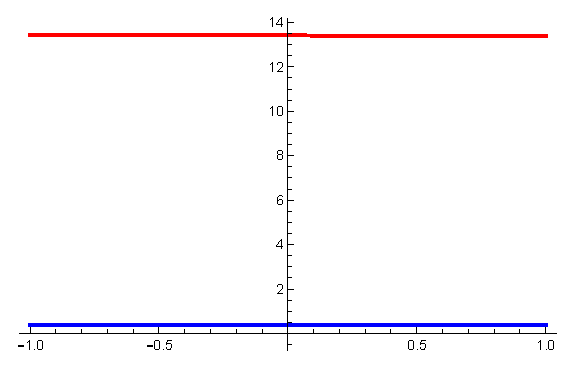
\includegraphics[width=0.7\textwidth]{graph1}
			\caption{График функций СЛАУ (1)}
			\label{graph1}
		\end{figure}	
		
		\item \textbf{Вопрос №8 (Подсчитать число операций в модифицированном матоде Гаусса)}
		
		Поскольку модифицированная схема не уменьшает количество операций на этапе прямого хода, общая сложность остаётся $O(n^3)$. Основное преимущество~-- это оптимизация по числу операций ввода-вывода и экономия времени за счёт совмещения процессов. Но с точки зрения арифметической сложности, модифицированная схема метода Гаусса остаётся такой же, как и классический метод -- $O(n^3)$.
		
		\item \textbf{Вопрос №10 (Какие нормы называются эквивалентными? Картинки норм)}
		
		Две нормы $p$ и $q$, заданные на пространстве $V$ называются \textbf{эквивалентными}, если 
		$\forall x \in V, \exists \alpha,\beta \in \mathbb{R}: \alpha p(x) \le q(x) \le \beta p(x)$.
		
		\begin{figure}[!h]
			\center
			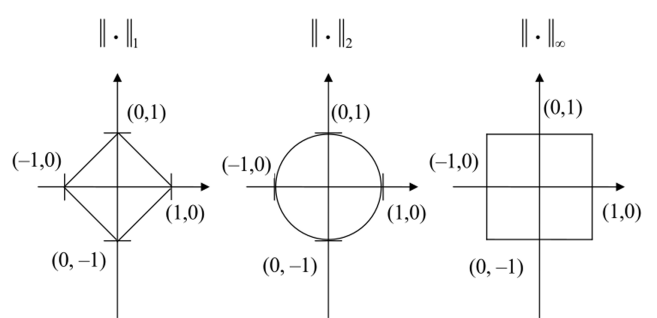
\includegraphics[width=0.7\textwidth]{pic1}
			\caption{Нормы}
			\label{pic1}
		\end{figure}		
		
	\end{enumerate}
	
	
\end{document} 